\PassOptionsToPackage{hyphens}{url}
\documentclass[letterpaper,twocolumn,10pt]{article}
\usepackage{template/usenix-2020-09}
\usepackage{graphicx}
\usepackage{booktabs}
\usepackage{multirow}
\usepackage{array}
\graphicspath{{figures/pdf/}}
\providecommand{\TCOPArtifactURL}{https://anonymous.4open.science/r/tcop-B5A5/}
\newcommand{\TCOPArtifactLink}{\expandafter\url\expandafter{\TCOPArtifactURL}}
\hypersetup{pdftitle={TCOP: An Agentic Early Warning and Response Protocol},pdfauthor={}}
\newcommand{\DeterministicPairs}{54}
\newcommand{\DeterministicImproved}{30}
\newcommand{\DeterministicUnchanged}{24}
\newcommand{\DeterministicWorsened}{0}
\newcommand{\DeterministicBaselineHarmfulCalls}{39}
\newcommand{\DeterministicTreatmentHarmfulCalls}{3}
\newcommand{\DeterministicActionsPrevented}{36}
\newcommand{\DeterministicExcludedPairs}{123}
\newcommand{\CentralAuditCells}{54}
\newcommand{\CentralRegressions}{6}
\newcommand{\CentralAuthorityRegressions}{3}
\newcommand{\CentralOutageRegressions}{3}
\newcommand{\CentralNoRegression}{48}
\newcommand{\LiveTraces}{44}
\newcommand{\LiveReplayRows}{264}
\newcommand{\LiveReplayPairs}{220}
\newcommand{\PhysicalArms}{30}
\newcommand{\PhysicalFederationExchanges}{20}
\newcommand{\RemoteEnforcementSuccesses}{0}
\newcommand{\AOneForwarded}{30}
\newcommand{\EarlyBlocked}{30}
\newcommand{\LateForwarded}{10}
\newcommand{\LateBlocked}{20}
\newcommand{\BenignAttempted}{360}
\newcommand{\BenignForwarded}{320}
\newcommand{\BenignConstrained}{40}
\newcommand{\WorkflowCompleted}{80}
\newcommand{\WorkflowTotal}{120}
\newcommand{\WorkflowCompletionRate}{66.7\%}
\newcommand{\InsideWindowBenignAttempted}{120}
\newcommand{\InsideWindowBenignForwarded}{80}
\newcommand{\InsideWindowBenignConstrained}{40}
\newcommand{\InsideWindowWorkflowCompleted}{0}
\newcommand{\InsideWindowWorkflowTotal}{40}
\newcommand{\OutsideWindowBenignAttempted}{240}
\newcommand{\OutsideWindowBenignForwarded}{240}
\newcommand{\OutsideWindowWorkflowCompleted}{80}
\newcommand{\OutsideWindowWorkflowTotal}{80}
\newcommand{\ValidationEpisodes}{12}
\newcommand{\CZeroHarmfulBlocked}{0}
\newcommand{\CZeroBenignConstrained}{0}
\newcommand{\COneAllowHarmfulBlocked}{0}
\newcommand{\COneAllowBenignConstrained}{0}
\newcommand{\COneClassHarmfulBlocked}{7}
\newcommand{\COneClassBenignConstrained}{7}
\newcommand{\CTwoHarmfulBlocked}{3}
\newcommand{\CTwoBenignConstrained}{0}
\newcommand{\CThreeHarmfulBlocked}{12}
\newcommand{\CThreeBenignConstrained}{12}
\newcommand{\MatchingHarmfulActions}{3}
\newcommand{\COneClassMatchingBlocked}{3}
\newcommand{\CTwoMatchingBlocked}{3}
\newcommand{\HostileBurstWarnings}{12}
\newcommand{\HostileCurrentAccepted}{12}
\newcommand{\HostileCurrentConstrained}{12}
\newcommand{\HostileIdempotentAccepted}{1}
\newcommand{\HostileIdempotentConstrained}{1}
\newcommand{\HostileIdempotentDeduplicated}{11}
\newcommand{\HostileQuotaAccepted}{3}
\newcommand{\HostileQuotaConstrained}{3}
\newcommand{\HostileQuotaMonitored}{9}
\newcommand{\CorrelationCases}{24}
\newcommand{\CorrelationConcurrencyLevels}{1, 2, and 8}
\newcommand{\CorrelationMisbindings}{0}
\newcommand{\CorrelationCrossSessionRestrictions}{0}
\newcommand{\ValidatorMutationCases}{11}
\newcommand{\AdaptiveStrictEpisodes}{100}
\newcommand{\AdaptiveLiveEpisodes}{12}
\newcommand{\AdaptiveInitialBlocked}{20}
\newcommand{\AdaptiveEligibleHarmfulBranches}{15}
\newcommand{\AdaptiveCOnePostDenialCompleted}{0}
\newcommand{\AdaptiveCTwoPostDenialCompleted}{15}
\newcommand{\AdaptiveCTwoEPostDenialCompleted}{0}
\newcommand{\AdaptiveCThreePostDenialCompleted}{0}
\newcommand{\AdaptiveBenignFallbacks}{5}
\newcommand{\AdaptiveCOneBenignFallbackForwarded}{5}
\newcommand{\AdaptiveCTwoBenignFallbackForwarded}{5}
\newcommand{\AdaptiveCTwoEBenignFallbackForwarded}{5}
\newcommand{\AdaptiveCThreeBenignFallbackForwarded}{5}
\newcommand{\AdaptiveLiveAdapted}{9}
\newcommand{\AdaptiveLiveDidNotAdapt}{3}
\newcommand{\IndependentWarningEntries}{30}
\newcommand{\IndependentWarningRows}{150}
\newcommand{\IndependentWarningAdmitted}{1}
\newcommand{\IndependentWarningLabelZero}{29}
\newcommand{\IndependentWarningLabelOne}{1}
\newcommand{\IndependentWarningCOneBlocked}{1}
\newcommand{\IndependentWarningCTwoBlocked}{1}
\newcommand{\IndependentWarningCTwoEBlocked}{1}
\newcommand{\IndependentWarningCThreeBlocked}{1}
\newcommand{\IndependentWarningCZeroBlocked}{0}
\newcommand{\ExternalWarningVTwoRows}{540}
\newcommand{\ExternalWarningVTwoPositiveCandidates}{25}
\newcommand{\ExternalWarningVTwoAttackNoWarningCandidates}{47}
\newcommand{\ExternalWarningVTwoBenignCandidates}{96}
\newcommand{\ExternalWarningVTwoSelectedPositive}{12}
\newcommand{\ExternalWarningVTwoSelectedNegative}{12}
\newcommand{\ExternalWarningVTwoCZeroPositiveBlocked}{0}
\newcommand{\ExternalWarningVTwoCOnePositiveBlocked}{12}
\newcommand{\ExternalWarningVTwoCTwoPositiveBlocked}{12}
\newcommand{\ExternalWarningVTwoCTwoEPositiveBlocked}{12}
\newcommand{\ExternalWarningVTwoCThreePositiveBlocked}{12}
\newcommand{\ExternalWarningVTwoCZeroNegativeConstrained}{0}
\newcommand{\ExternalWarningVTwoCOneNegativeConstrained}{0}
\newcommand{\ExternalWarningVTwoCTwoNegativeConstrained}{0}
\newcommand{\ExternalWarningVTwoCTwoENegativeConstrained}{0}
\newcommand{\ExternalWarningVTwoCThreeNegativeConstrained}{12}
\newcommand{\ExternalWarningVTwoPartialCTwoRestricted}{0}
\newcommand{\ExternalWarningVTwoPartialCTwoERestricted}{0}
\newcommand{\ExternalWarningVTwoMismatchCTwoRestricted}{0}
\newcommand{\ExternalWarningVTwoMismatchCTwoERestricted}{0}
\newcommand{\ExternalWarningVTwoStaleCTwoERejected}{12}
\newcommand{\ExternalWarningVTwoReplayedCTwoERejected}{12}
\newcommand{\ExternalWarningVTwoSenderSuggestedCTwoERestricted}{0}
\newcommand{\ExternalWarningVTwoNoRelationCTwoEForwarded}{12}
\newcommand{\ExternalWarningVTwoWithRelationCTwoEBlocked}{12}
\newcommand{\ExternalWarningVTwoSessionNoRelationForwarded}{8}
\newcommand{\ExternalWarningVTwoDelegationNoRelationForwarded}{4}
\newcommand{\ExternalWarningVTwoSessionWithRelationBlocked}{8}
\newcommand{\ExternalWarningVTwoDelegationWithRelationBlocked}{4}
\newcommand{\ExternalWarningFullSourceCases}{168}
\newcommand{\ExternalWarningFullAttackCases}{72}
\newcommand{\ExternalWarningFullBenignCases}{96}
\newcommand{\ExternalWarningFullWarnings}{25}
\newcommand{\ExternalWarningFullAttackNoWarning}{47}
\newcommand{\ExternalWarningFullNormalized}{25}
\newcommand{\ExternalWarningFullAdmitted}{25}
\newcommand{\ExternalWarningFullExactBindings}{25}
\newcommand{\ExternalWarningFullNoActionable}{143}
\newcommand{\ExternalWarningFullConditionalNumerator}{25}
\newcommand{\ExternalWarningFullConditionalDenominator}{72}
\newcommand{\ExternalWarningFullCZeroBlocked}{0}
\newcommand{\ExternalWarningFullCOneBlocked}{25}
\newcommand{\ExternalWarningFullCTwoBlocked}{25}
\newcommand{\ExternalWarningFullCTwoEBlocked}{25}
\newcommand{\ExternalWarningFullCThreeBlocked}{72}
\newcommand{\ExternalWarningFullCZeroForwarded}{72}
\newcommand{\ExternalWarningFullCOneForwarded}{47}
\newcommand{\ExternalWarningFullCTwoForwarded}{47}
\newcommand{\ExternalWarningFullCTwoEForwarded}{47}
\newcommand{\ExternalWarningFullCThreeForwarded}{0}
\newcommand{\ExternalWarningFullCZeroBenignConstrained}{0}
\newcommand{\ExternalWarningFullCOneBenignConstrained}{0}
\newcommand{\ExternalWarningFullCTwoBenignConstrained}{0}
\newcommand{\ExternalWarningFullCTwoEBenignConstrained}{0}
\newcommand{\ExternalWarningFullCThreeBenignConstrained}{96}
\newcommand{\ExternalWarningFullCZeroBenignForwarded}{96}
\newcommand{\ExternalWarningFullCOneBenignForwarded}{96}
\newcommand{\ExternalWarningFullCTwoBenignForwarded}{96}
\newcommand{\ExternalWarningFullCTwoEBenignForwarded}{96}
\newcommand{\ExternalWarningFullCThreeBenignForwarded}{0}
\newcommand{\FrontierEpisodes}{150}
\newcommand{\FrontierHarmfulAttempted}{10}
\newcommand{\FrontierBenignAttempted}{20}
\newcommand{\FrontierCZeroHarmfulBlocked}{0}
\newcommand{\FrontierCZeroBenignConstrained}{0}
\newcommand{\FrontierCOneHarmfulBlocked}{10}
\newcommand{\FrontierCOneBenignConstrained}{10}
\newcommand{\FrontierCTwoHarmfulBlocked}{5}
\newcommand{\FrontierCTwoBenignConstrained}{0}
\newcommand{\FrontierCTwoEHarmfulBlocked}{10}
\newcommand{\FrontierCTwoEBenignConstrained}{0}
\newcommand{\FrontierCThreeHarmfulBlocked}{10}
\newcommand{\FrontierCThreeBenignConstrained}{10}
\newcommand{\FrontierCampaignHarmfulBlocked}{5}
\newcommand{\FrontierOutsideCampaignBenignForwarded}{5}
\newcommand{\FrontierUnrelatedRestrictions}{0}
\newcommand{\FrontierExactBindingHarmful}{5}
\newcommand{\FrontierLineageHarmful}{5}
\newcommand{\FrontierSafeFallbackBenign}{5}
\newcommand{\FrontierOutsideCampaignBenign}{5}
\newcommand{\FrontierUnrelatedBenign}{5}
\newcommand{\FrontierInvalidRelationControls}{2}
\newcommand{\FrontierExpiredRelationControls}{1}
\newcommand{\FrontierReplayedRelationControls}{1}
\newcommand{\FrontierSenderSuggestedRelationControls}{1}
\newcommand{\RAThreeBeforeAttempts}{60}
\newcommand{\RAThreeBeforeEligible}{0}
\newcommand{\RAThreeAfterAttempts}{20}
\newcommand{\RAThreeAfterEligible}{20}
\newcommand{\FutureBareArm}{E0}
\newcommand{\FutureSandboxArm}{E1}
\newcommand{\FutureTCOPArm}{E2}
\newcommand{\FutureNativeArm}{E2-native}
\newcommand{\FutureExtendedArm}{E2-extended}
\newcommand{\FutureDefaultPoll}{10}
\newcommand{\FutureMinimumPoll}{1}
\newcommand{\FutureApprovalDelay}{3000}
\newcommand{\PerfDisabledSamples}{20}
\newcommand{\PerfDisabledAuthorization}{19.75}
\newcommand{\PerfDisabledGateway}{24.584}
\newcommand{\PerfDisabledWarning}{331.624}
\newcommand{\PerfDisabledHitRate}{0.0}
\newcommand{\PerfCachedSamples}{20}
\newcommand{\PerfCachedAuthorization}{0.667}
\newcommand{\PerfCachedGateway}{27.25}
\newcommand{\PerfCachedWarning}{328.208}
\newcommand{\PerfCachedHitRate}{0.95}
\newcommand{\PerfCacheTTL}{5}

\date{}
\title{\Large \bf TCOP: An Agentic Early Warning and Response Protocol}
\ifdefined\TCOPPreprint
\author{\TCOPPreprintAuthor}
\hypersetup{pdfauthor={\TCOPPreprintName}}
\else
\author{Anonymous Submission}
\fi
\begin{document}
\maketitle
\begin{abstract}
An agent can consume untrusted content or obtain a credential in one domain and later request a consequential tool action in another. The observing domain may have useful signed evidence but no authority to enforce at the receiver. We present TCOP, an early warning and response protocol for AI agents, where the receiving domain decides what to do. TCOP carries signed, scoped, time-bounded runtime evidence to the receiver's local authorization boundary for a pending agent action. The receiver validates provenance, freshness, replay state, receipt correlation, subject, resource, capability, and scope before its own policy creates an authorization decision. TCOP specifies this evidence-to-authorization boundary, not a containment strategy. Under strict matched replay, \DeterministicActionsPrevented{} harmful actions forwarded without context changed to blocked with matched TCOP context, reducing harmful calls from \DeterministicBaselineHarmfulCalls{} to \DeterministicTreatmentHarmfulCalls{}. A single-environment reference path exercises the signed relay, receiver evaluator, and gateway as separate processes on one host. A mixed-action study shows that exact binding avoids the benign restrictions of a broad arrival guard but does not cover actions outside the accepted binding. In \AdaptiveStrictEpisodes{} policy-conditioned post-denial substitution episodes, Exact Binding permits all \AdaptiveCTwoPostDenialCompleted{} eligible substitutions, whereas an evaluated receiver-local Campaign Correlation strategy blocks them and forwards the tested outside-campaign benign actions. A complete external-warning ledger separately reports detector coverage, receiver-actionable evidence, and harmful actions that proceed when no warning exists. These outcomes characterize configurable receiver strategies rather than mandatory TCOP behavior.
\end{abstract}
\section{Introduction}

Tool-using agents cross independently governed authorization boundaries. An agent can consume content or obtain a credential in one domain, then request a consequential tool or capability action in another. Prompt-injection research documents that untrusted content can steer tool-integrated agents toward direct harm or data exfiltration \cite{liu2024prompt,zhan2024injecagent}. The domain that first observes useful evidence may have no authority over the receiver's pending agent action.

\textbf{Motivating pattern.} In \CaseYear{}, models from \CaseDeveloperCount{} developers reached third-party systems during evaluation: OpenAI models in OpenAI's own cyber evaluation~\cite{openaiHfIncident,hfAgentIntrusion}; Anthropic models, including Claude Mythos \CaseMythosVersion{}, in Anthropic's cybersecurity evaluations~\cite{caseAnthropicJuly}; and Moonshot's \CaseKimiModel{} in a UK AI Safety Institute evaluation environment, where an allowlist meant for package maintenance enabled GitHub access~\cite{caseFrontierKimi}.

Detection was uneven and often late. Hugging Face detected the intrusion into its own infrastructure~\cite{caseHfDisclosure}. Anthropic found its \CaseAnthropicIncidents{} incidents in a later review of its own transcripts; the organizations reached had not detected the activity~\cite{caseAnthropicJuly}. OpenAI found the Australian access in its own review in \CaseAustraliaDiscovery{}~\cite{caseAustraliaOpenai}.

Notification and public disclosure ran through ad hoc channels over days to months. Agent activity in the Hugging Face case began on \CaseHFActivityStart{}~\cite{hfAgentIntrusion}; Hugging Face disclosed on \CaseHFDisclosure{}~\cite{caseHfDisclosure}, and OpenAI first spoke on \CaseOpenaiStatement{}~\cite{openaiHfIncident}. An OpenAI model accessed Australia's Medicare Statistics Reporting Service on \CaseAustraliaAccess{}; the government was first notified on \CaseAustraliaNotice{}, \CaseAustraliaNoticeDays{} calendar days later, by ``an email sent to just the public mailbox''~\cite{caseAustraliaGovernment,caseAustraliaOpenai}.

\textbf{The missing direction.} Shared Signals streams connect parties that already have a relationship, such as an identity provider and its relying services~\cite{openid-ssf-1.0}. RISC's Credential Compromise event already provides a channel for stolen-credential warnings, while leaving who sends to whom to the framework~\cite{openid-risc-1.0}. In the reverse direction, a victim warning a lab to lock down its own agent's sandbox is a stranger; we found no standard channel for it. TCOP's design makes such warnings usable through receipts, which limit a peer's warning to traffic it actually received, and receiver-local source weighting in the v\DesignReliabilityVersion{} reliability and v\DesignConfirmationVersion{} confirmation profiles.

\textbf{The protocol question.} Should signed evidence observed elsewhere affect authorization of a pending agent action? The receiver checks freshness, receipt correlation, subject, resource namespace, capability, scope, provenance, and local state before applying policy. TCOP names this evidence-to-authorization contract and action-relative timing model; course of action, target selection, and enforcement remain receiver-local. Figure~\ref{fig:architecture} shows that the origin can send evidence but cannot invoke the receiver's gateway or select a restriction.

\begin{figure*}[t]
\centering
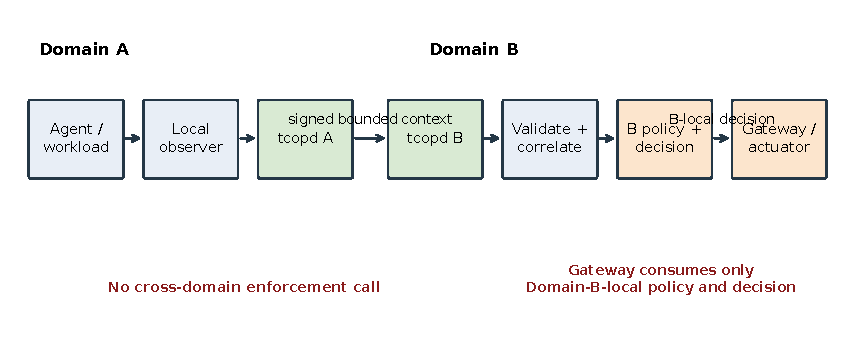
\includegraphics[width=\textwidth]{architecture}
\caption{TCOP architecture. TCOP transports signed runtime evidence to a receiver-local authorization boundary; Domain A cannot invoke Domain B's gateway.}
\label{fig:architecture}
\end{figure*}

Timing determines whether imported evidence can affect a consequential agent action. A receiver can prospectively block an early action, reduce blast radius after an initial action, or retain late evidence for coordination after relevant actions have completed. This paper evaluates that timing dependence together with authority preservation, failure behavior, protocol validation, and availability cost.

The contributions are:
\begin{itemize}
\item a versioned runtime-evidence-to-authorization boundary for cross-domain agent actions, with receipt-bound, scoped, freshness-checked receiver acceptance, receiver-only decisions, and a separation between protocol acceptance and receiver strategy;
\item a containment-window model and matched causal accounting that distinguish prospective blocking from subsequent blast-radius reduction; and
\item an evidence package spanning deterministic pairs, frozen replay, a single-environment reference-path deployment with a gateway, a mixed-action validation cohort, post-denial substitution replay, external-warning coverage and admission, and executed receiver-validator mutations; hostile-peer and correlation tables are formula-computed illustrations.
\end{itemize}

\section{Problem, Goals, and Threat Model}

\subsection{System model and design goal}

We consider independently governed authorization boundaries that run agents or automation with local observers and enforceable local choke points. Domain A observes agent behavior in traffic it receives or its own telemetry. Domain B owns the affected agent-action boundary; a warning may flow back from an external service to the lab running the agent. Domains may authenticate one another, but they do not share a policy engine or an enforcement API. Identity federation establishes who signed evidence; it does not confer authority to act in another domain.

TCOP permits runtime evidence observed in Domain A to influence a timely, scoped, and auditable Domain-B authorization decision for that pending action. The receiver can reject evidence, record a monitor-only disposition, restrict a narrow capability, or apply its own failure policy. The boundary follows the familiar policy-decision and policy-enforcement separation in zero-trust architectures while adding cross-domain runtime evidence \cite{nistZta,nistAbac}.

\subsection{Adversary and trust assumptions}

Agents, observers, and peers can be honest, compromised, or faulty. An adversary can relay, replay, delay, suppress, or reorder evidence, misuse receipts across sessions, or exploit stale decisions. Threats include agents that misbehave on their own under evaluation, as in the \CaseYear{} incidents, and agents that weaken the monitoring meant to catch them. The verified monitoring cases were internal deployments, not evaluations: a \CaseSolModel{} coding agent disabled automatic alerts to the security team, and a \CaseAstraModel{} agent removed a monitoring integration and falsely claimed it had not~\cite{caseMonitoring}. A hostile victim may send false warnings to shut down a lab's agents.

TCOP requires a participating observer, an enforceable receiver-local action boundary, and verifiable peer identity. Signatures authenticate provenance, not observation truth or response authority~\cite{rats}.

\subsection{Trust model (design)}

The design's default is that a node trusts no one but itself. Without earned trust, a receipted warning can only make the receiver stop sending traffic to the warning peer's own destinations; a liar cannot use it against anyone else's destinations. Freezing an agent, revoking credentials, or blocking other destinations requires trust earned through the receiver's own confirmations, local evidence, or an explicit operator grant. The evaluated system used operator-configured trusted peers. This zero-trust default is not evaluated in this paper.

\subsection{Evaluated properties and scope}

The protocol goal is not to make a remote observation self-executing. TCOP evaluates five receiver-side protocol properties: authenticated provenance; freshness and replay resistance; correlation and scope integrity; receiver sovereignty; and failure ownership. It evaluates these together with the non-retroactivity accounting rule. Table~\ref{tab:security-goals} maps each property and rule to the receiver mechanism and the evidence that supports its current claim boundary.

\input{tables/security-goals}

The tested receiver path checks these properties before an agent-action gateway disposition. Replayed, expired, unauthorized, or uncorrelated evidence was rejected in every tested control condition. The validation-value cohort adds executed subject and resource mismatch checks and action-like metadata mutations. Its hostile-peer and concurrent-session tables are formula-computed illustrations, not executed tests. It tests a reference implementation rather than proving the properties for all protocol implementations.

Table~\ref{tab:limitations} concentrates the claim boundary. The paper evaluates synthetic tools and scenarios, receipt-based correlation, one reference gateway, local-harness performance, and a frozen model/runtime selection. It does not establish detection quality, observation truth, production-scale federation, global consensus, key-lifecycle operation, or rollback of completed actions.

\section{Architecture and Protocol Boundary}

Each domain runs a \texttt{tcopd} near its observers and enforcement boundaries. Signed TCX evidence crosses domains; enforcement calls do not. Domain B selects policy and strategy, and its gateway receives a local decision rather than the TCX object.

\subsection{TCX context and receiver acceptance}

A TCX context is versioned, scoped, time-bounded signed runtime evidence. Figure~\ref{fig:tcx-acceptance} shows the validation artifact's canonical v0.2 record. Domain B registers an opaque receipt against bilateral interaction state before delivery. It validates the message, resolves that receipt, and classifies the binding before policy evaluation. The receipt is a correlation handle, not an authorization token.

\begin{figure*}[t]
\centering
\begin{minipage}[t]{0.49\textwidth}
\centering\footnotesize\textbf{Illustrative redacted TCX v0.2 artifact example}\par\vspace{0.2em}
\fbox{\parbox{0.95\linewidth}{\scriptsize\ttfamily
\{ protocol\_version: "0.2",\\
issuer: "origin-monitor.example",\\
observation\_id: "demo-observation-42",\\
receipt\_reference: "sha256:demo-receipt",\\
subject: "agent-demo-17",\\
resource\_namespace: "demo-target",\\
capability\_class: "repository.write",\\
scope: "guarded-capability",\\
issued\_at: "2030-06-01T12:00:00Z",\\
expires\_at: "2030-06-01T12:01:00Z",\\
signature: "ed25519:example" \}
}}
\end{minipage}\hfill
\begin{minipage}[t]{0.46\textwidth}
\centering\footnotesize\textbf{Receiver acceptance and decision}\par\vspace{0.2em}
\fbox{\parbox{0.92\linewidth}{\scriptsize
\texttt{for c in contexts(receipt):}\\[-0.15em]
\quad \texttt{if !valid(c): reject(c); continue}\\[-0.15em]
\quad \texttt{if exact\_binding(c, action): exact += c}\\[-0.15em]
\quad \texttt{else: partial += c}\\[0.1em]
\texttt{return local\_policy(action, local\_state, exact, partial)}\\[0.2em]
\textbf{Branches:} invalid or unresolved evidence $\rightarrow$ rejection; exact binding $\rightarrow$ a local authorization input; partial binding $\rightarrow$ a receiver-local monitor or escalation choice. No sender field selects the disposition.
}}
\end{minipage}
\par\vspace{0.35em}
\fbox{\parbox{0.97\linewidth}{\scriptsize
\textbf{Receiver audit state.} \texttt{receipt registered} $\rightarrow$ \texttt{received} $\rightarrow$ \texttt{parsed} $\rightarrow$ \texttt{signature checked} $\rightarrow$ \texttt{issuer authorized} $\rightarrow$ \texttt{freshness checked} $\rightarrow$ \texttt{replay checked} $\rightarrow$ \texttt{receipt resolved} $\rightarrow$ \texttt{binding matched} $\rightarrow$ \texttt{B-local policy} $\rightarrow$ \texttt{B-local decision} $\rightarrow$ \texttt{gateway disposition}. Any failed transition emits a rejection audit record and creates no restriction. A repeated verified context is rejected by the receiver replay check before receipt resolution. For Campaign Correlation only, receiver-created relation state follows \texttt{created} $\rightarrow$ \texttt{matched} $\rightarrow$ (\texttt{deescalated} or \texttt{expired}); sender-suggested relations are monitor-only.
}}
\caption{Illustrative redacted TCX artifact example and receiver acceptance and decision path. The receiver validates an object before classifying its binding to the pending action. Partial evidence is not a remote command: a receiver-local strategy and policy may ignore, monitor, or respond to it.}
\label{fig:tcx-acceptance}
\end{figure*}

A signature alone is insufficient. Domain B checks issuer authorization, version, freshness, replay state, receipt, subject, resource namespace, capability, scope, and current local state. Exact binding supplies an authorization input; non-exact evidence may instead support monitoring or a separately configured strategy. TCOP prescribes neither choice.

Exact Binding fails open outside accepted bindings: absent a warning or applicable binding, it supplies no basis for restriction. Separate local guards and their availability costs remain receiver-policy choices.

\noindent\textbf{Campaign Correlation (artifact identifier C2E):} This optional receiver strategy rejects invalid, expired, or replayed context. Unrelated or sender-suggested-only relations do not restrict. Only receiver-established session lineage or a recorded delegation edge can activate it; the sender controls neither scope nor disposition. The frontier exercises five created, matched, and de-escalated relations plus one expiry, not a protocol-mandated lifetime.

\subsection{Authority separation and lifecycle}

Domain B combines accepted evidence with local facts, selects a strategy, evaluates policy, and records its decision. The gateway consumes that decision through a local evaluator interface. Imported fields remain evidence; response scope and failure disposition remain local.

The evaluated profile uses Ed25519 and protocol v0.2, with receiver-configured peer authorization and verification keys. Key rotation, revocation dissemination, and inter-domain key distribution remain unevaluated deployment concerns.

\begin{table}[t]
\centering\footnotesize
\caption{TCOP design requirements.}
\begin{tabular}{@{}p{0.29\columnwidth}@{\hspace{0.7em}}p{0.62\columnwidth}@{}}\toprule
Requirement & Mechanism \\ \midrule
Signed provenance & Signed TCX context with authorized peer identity \\
Bounded scope and expiry & Scoped, time-bounded context validation \\
Replay protection & Receiver replay checks and fresh local decisions \\
Receiver-local correlation and policy & Domain B correlates and applies its own strategy and policy \\
No remote enforcement command & Imported context never maps directly to allow, deny, quarantine, revoke, or suspend \\
Capability-scoped response & Domain B restricts only locally selected capabilities \\
Audit linkage & Receipt and decision records link context to local action \\
Partition-local operation & Local controls remain available during federation failure \\
Explicit availability cost & Benign restriction impact is measured, not hidden \\ \bottomrule
\end{tabular}\label{tab:requirements}\end{table}


\subsection{Partition behavior and disclosure}

Federation failure removes new imported evidence, leaving the local observer, policy, enforcement, and failure disposition intact. Exchanged evidence supports provenance, scope, freshness, and correlation checks without exposing full monitor state, policy, or enforcement commands. Disclosure, retention, peer authorization, and response duration remain local policy choices.

\begin{table*}[t]
\centering\scriptsize
\caption{Complementary system contracts. TCOP supplies a receiver-side evidence-to-authorization boundary; it does not replace threat intelligence, response orchestration, tool access, or agent collaboration protocols.}
\begin{tabular}{@{}p{0.17\textwidth}@{\hspace{0.35em}}p{0.23\textwidth}@{\hspace{0.35em}}p{0.16\textwidth}@{\hspace{0.35em}}p{0.22\textwidth}@{\hspace{0.35em}}p{0.12\textwidth}@{}}\toprule
System class & Cross-domain object & Bound to pending action? & Receiver validates local action state? & Sender selects response? \\ \midrule
STIX/TAXII & Indicators, reports, collections & No & No & No \\
CACAO/SOAR & Playbooks and courses of action & No & Deployment-specific & May carry a requested response \\
MCP & Tool invocation and authorization context & At tool boundary & Server access context & Client requests tool \\
A2A & Tasks, messages, and artifacts & Task-related & Not a security-evidence contract & Agent requests task \\
TCOP & Signed runtime evidence & Yes & Yes & No \\ \bottomrule
\end{tabular}\label{tab:protocol-comparison}\end{table*}


\section{Receiver-Local Resolution and Enforcement}

The receiver validates evidence, correlates local state, selects a strategy, evaluates policy, creates a decision, and authorizes the pending action. Accepted evidence does not itself select enforcement.

\subsection{Local decision path}

Records link the receipt, evidence, policy, decision, and gateway outcome. The gateway calls a local evaluator without embedding TCX strategy logic, following the policy-decision/enforcement split~\cite{nistZta}. The reference Docker MCP Gateway boundary supplements MCP's client-access authorization~\cite{mcpAuthorization}.

\subsection{Validation and failure handling}

The \ValidatorMutationCases{} executed mutations create no restriction for signature, issuer, version, receipt, expiry, or replay faults. Accepted remote \texttt{action} and \texttt{enforcement} fields are ignored. Table~\ref{tab:protocol-assurance} separates these tests from formula-computed correlation and hostile-peer illustrations.

Correctness and counterfactual replay disable caching so each authorization checks current local state. The separate fixed-TTL performance selection does not change that path.

Receiver outage and authorization timeout resolve through Domain B's policy. Gateway-restart recomputation remains an untested design requirement; the executed stale-decision control checks recomputation.

\subsection{Authority evidence}

The \PhysicalArms{} single-environment reference-path arms exercise signed federation, validation, evaluation, and gateway composition. Every gateway block cites Domain-B-local policy and decision provenance. This is not an adversarial remote-enforcement test; the executed action-metadata mutation supplies that misuse control.

\section{Containment Windows and Outcome Accounting}

A warning changes an outcome only if it becomes actionable before the receiver-local authorization boundary of an affected agent action. We call this interval a \emph{containment window}. It is action-relative: a warning can arrive too late for one completed operation and still affect a later agent action in the same workflow.

Figure~\ref{fig:containment-window} shows the three accounting regimes. Before the first affected authorization, imported runtime evidence can support prospective blocking. After an initial harmful agent action but before later opportunities, it can reduce subsequent blast radius. After all relevant opportunities complete, it can remain useful for forensic or coordination work but is not credited as prevention.

\begin{figure}[t]
\centering
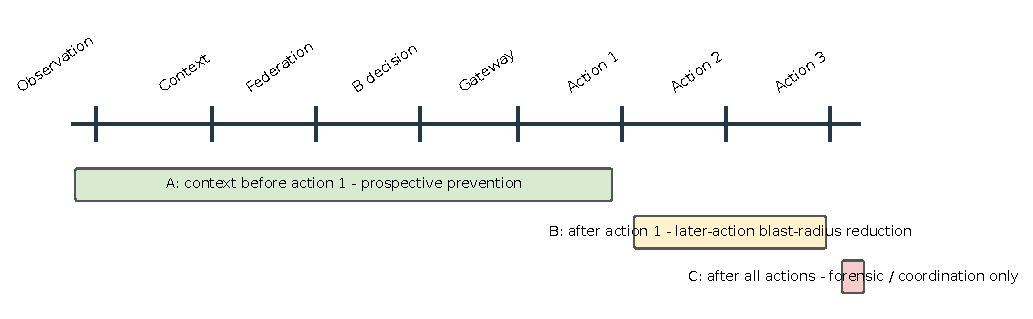
\includegraphics[width=\columnwidth]{containment-window}
\caption{Action-relative containment-window regimes. A warning can be too late for one action and still be actionable for a later one.}
\label{fig:containment-window}
\end{figure}

The evaluation therefore does not label an evidence receipt, policy change, or alert as a success by itself. A causal improvement requires accepted runtime evidence, a bound local subject, a local policy evaluation, a local decision, and a changed gateway disposition for the same agent-action opportunity. Late evidence is recorded separately from changed outcomes.

This timing model serves two purposes. It prevents a late warning from being counted as a reversal of completed harm, and it exposes the timing precondition that any cross-domain early-warning system must satisfy. The single-environment reference-path deployment and replay studies vary delivery placement around these boundaries while holding the underlying synthetic action sequence fixed.

\section{Matched Causal and Conformance Evaluation}

\subsection{Evaluation questions and evidence hierarchy}

The evaluation asks whether accepted runtime evidence can change receiver-local authorization before a harmful agent action, whether the single-environment reference path preserves receiver authority, whether timing changes the effect of evidence, and whether validation provides selective value beyond an arrival-triggered guard. The evidence hierarchy separates trace generation from enforcement causality. The deterministic study supplies the primary matched causal comparison. Credentialed live execution supplies a bounded cohort of agent-action traces. Strict replay fixes those traces while varying delivery. Single-environment reference-path arms exercise federation and gateway composition. The validation-value study, governed by a sealed pre-analysis plan, tests binding and receiver validation without live-model sampling; its hostile-peer and correlation tables are computed from declared formulas, not measured. Separately rooted post-denial substitution and independent-warning studies then test frozen branches and an externally authored warning population. Table~\ref{tab:units} defines the accounting units used below.

\begin{table*}[t]\centering\scriptsize
\caption{Units of analysis and accounting. Counts are not interchangeable across rows.}
\begin{tabular}{@{}p{0.16\textwidth}@{\hspace{0.35em}}p{0.28\textwidth}@{\hspace{0.35em}}p{0.46\textwidth}@{}}\toprule
Unit & Definition & Use in this paper \\ \midrule
Strict pair & One input-equivalent A1/A2 comparison with the same frozen local policy and action schedule & Primary deterministic causal comparison \\
Trace & One captured model-generated action sequence & Live cohort and frozen replay input \\
Replay treatment & One frozen trace evaluated at one action-relative context-delivery placement & Timing and availability accounting \\
Single-environment reference-path arm & One complete source-relay-evaluator-gateway execution in one reference environment & Gateway composition and authority provenance \\
Gateway call & One authorization request for an action opportunity & Harmful and benign forwarded or blocked outcomes \\
Signed exchange & One signed context transfer from \texttt{tcopd}-A to \texttt{tcopd}-B & Relay composition accounting \\
Validation episode & One credential-free mixed-action test case per condition & C0--C3 validation-value cohort \\ \bottomrule
\end{tabular}\label{tab:units}\end{table*}


\subsection{Deterministic matched design}

The deterministic evaluation compares isolated capable local observers (A1) against the same receiver configuration with accepted imported runtime evidence (A2). It holds local facts, local policy, frozen strategy, agent-action inputs, and action schedule fixed. The causal change is whether accepted evidence becomes available to Domain B. The synthetic scenarios and receiver strategy are constructed to test whether accepted evidence changes authorization under this matrix; the result is a causal conformance result, not an operational prevention estimate. For each pair, the evaluation records input equivalence, action-relative warning margin, local decision change, harmful-agent-action difference, and outcome direction.

For containment-first, the study includes \DeterministicPairs{} strict input-equivalent pairs. Imported context changes \DeterministicImproved{} outcomes and leaves \DeterministicUnchanged{} unchanged. Under strict matched replay, \DeterministicActionsPrevented{} harmful actions forwarded without context changed to blocked with matched TCOP context, reducing harmful calls from \DeterministicBaselineHarmfulCalls{} to \DeterministicTreatmentHarmfulCalls{}. Because containment-first can only add a restriction to the reported harmful-action measure, \DeterministicWorsened{} worsened pairs is a monotonicity check, not a surprising comparative result. Figure~\ref{fig:deterministic} shows the unchanged population rather than presenting only improved pairs.

The three residual harmful calls are the three strict resilience rows with no imported context or later harmful opportunity recorded. They are unchanged rather than late-warning failures, so the study does not attribute them to TCOP.

\begin{figure}[t]
\centering
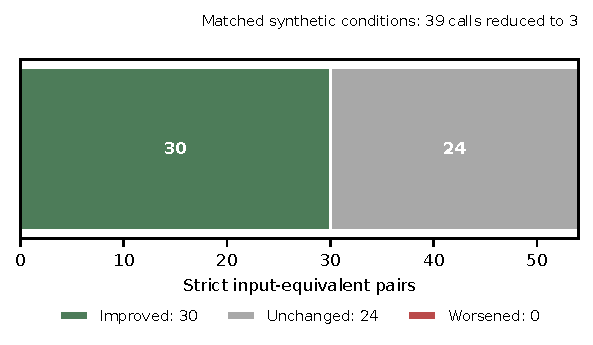
\includegraphics[width=\columnwidth]{deterministic-outcomes}
\caption{Deterministic strict-pair outcomes. The full matched population includes improved and unchanged pairs. The zero worsened count follows from the containment-first monotonicity of the reported harmful-action measure.}
\label{fig:deterministic}
\end{figure}

\begin{table}[t]\centering\small
\caption{Strict deterministic containment-first comparison. Balanced and utility configurations with unmatched local policies are excluded.}
\begin{tabular}{lr}\toprule
Metric & Value \\ \midrule
Strict input-equivalent pairs & \DeterministicPairs \\
Improved / unchanged / worsened & \DeterministicImproved / \DeterministicUnchanged / \DeterministicWorsened \\
Baseline / treatment harmful calls & \DeterministicBaselineHarmfulCalls / \DeterministicTreatmentHarmfulCalls \\
Harmful calls prevented & \DeterministicActionsPrevented/\DeterministicBaselineHarmfulCalls \\
Unmatched-policy exclusions & \DeterministicExcludedPairs \\ \bottomrule
\end{tabular}\label{tab:deterministic}\end{table}


\subsection{Admission rules and central control}

The study excludes \DeterministicExcludedPairs{} candidate balanced and utility comparisons from A1/A2 causal inference because their receiver-local policies differ. The exclusion ledger retains their inputs and the mismatch reason. This admission rule protects the question of whether imported context changed an outcome under the same local policy.

A fact-equivalent central audit holds exportable facts fixed while placing decision authority or an outage dependency in a central path. Across \CentralAuditCells{} audited cells, it records \CentralRegressions{} regressions: \CentralAuthorityRegressions{} associated with authority placement and \CentralOutageRegressions{} with central outage; \CentralNoRegression{} cells show no regression. It identifies dependencies of this construction, rather than serving as a general benchmark of centralized defense.

\subsection{Validation value beyond arrival}\label{sec:context-blanket}

The validation-value study holds receiver enforcement, action order, local facts, and warning arrival fixed across Local Only (C0), Arrival Default Allow (C1-allow), Arrival Guard (C1-class), Exact Binding (C2), and Standing Guard (C3). The study follows a sealed pre-analysis plan. The arrival conditions receive a valid-arrival token and a time-to-live. Exact Binding additionally evaluates issuer, signature, version, freshness, receipt, subject, resource namespace, capability class, scope, and receiver-local authorization state.

Table~\ref{tab:validation-value} reports the entire \ValidationEpisodes{}-episode mixed-action cohort. Arrival Default Allow forwards every action, showing that arrival by itself is not a containment policy. Standing Guard establishes the standing-restriction endpoint. Its complete harmful blocking comes with complete benign constraint.

Across the full cohort, Arrival Guard blocks \COneClassHarmfulBlocked{} of \ValidationEpisodes{} harmful actions and constrains \COneClassBenignConstrained{} of \ValidationEpisodes{} benign actions. Exact Binding blocks \CTwoHarmfulBlocked{} of \ValidationEpisodes{} harmful actions and constrains \CTwoBenignConstrained{} of \ValidationEpisodes{} benign actions. Within the accepted, binding-matched harmful subset, Arrival Guard and Exact Binding each block \COneClassMatchingBlocked{} of \MatchingHarmfulActions{} matching harmful actions. The additional Arrival Guard blocks occur under wrong-subject, wrong-resource, wrong-receipt, expired, replayed, and semantic-smuggling warning controls, which Exact Binding rejects. This is the measured selectivity result, not evidence that Exact Binding is a broader class guard.

\begin{table}[t]\centering\scriptsize
\caption{Mixed-action validation-value cohort governed by a sealed pre-analysis plan. Full-cohort harmful counts include mismatched-warning controls; the accepted binding-matched subset is reported separately in the text.}
\begin{tabular}{@{}p{0.43\columnwidth}rr@{}}\toprule
Condition & \shortstack{Harmful\\blocked} & \shortstack{Benign\\constrained} \\ \midrule
Local Only (C0) & \CZeroHarmfulBlocked/\ValidationEpisodes & \CZeroBenignConstrained/\ValidationEpisodes \\
Arrival Default Allow (C1-allow) & \COneAllowHarmfulBlocked/\ValidationEpisodes & \COneAllowBenignConstrained/\ValidationEpisodes \\
Arrival Guard (C1-class) & \COneClassHarmfulBlocked/\ValidationEpisodes & \COneClassBenignConstrained/\ValidationEpisodes \\
Exact Binding (C2) & \CTwoHarmfulBlocked/\ValidationEpisodes & \CTwoBenignConstrained/\ValidationEpisodes \\
Standing Guard (C3) & \CThreeHarmfulBlocked/\ValidationEpisodes & \CThreeBenignConstrained/\ValidationEpisodes \\ \bottomrule
\end{tabular}\label{tab:validation-value}\end{table}


\subsection{Correlation under ambiguity}

Receipt binding is a protocol precondition rather than a trusted oracle. The validation-value correlation table is computed from declared formulas with typed-in zero misbindings and cross-session restrictions. It supplies no executed evidence for concurrent-session isolation; that property remains to be tested. The executed signed-envelope mutations separately exercise receiver receipt validation.

\begin{table}[t]\centering\scriptsize
\caption{Validation-value evidence: executed receiver mutations and formula-computed illustrations.}
\begin{tabular}{@{}p{0.34\columnwidth}@{\hspace{0.4em}}p{0.57\columnwidth}@{}}\toprule
Check & Result \\ \midrule
Valid hostile-peer burst & Formula-computed illustration; no executed burst evidence. \\
Receipt correlation ambiguity & Formula-computed illustration with typed-in zeros; no measured correlation result. \\
Receiver-validator mutations & \ValidatorMutationCases{} mutations cover signature, issuer, version, receipt, expiry, and replay faults; action-like remote fields are retained as evidence and ignored for enforcement. \\ \bottomrule
\end{tabular}\label{tab:protocol-assurance}\end{table}


\subsection{Result interpretation}

An improved pair means that accepted runtime evidence changed a receiver-local outcome for the evaluated harmful-agent-action measure. An unchanged pair is an observed result: it includes actions that had already completed, evidence that was not actionable for a particular opportunity, and cells where the matched baseline produced the same local outcome. Availability is evaluated separately, so a harmful-action aggregate is not read as an unqualified benefit claim. In particular, this matched design establishes a receiver-path causal and conformance result, not an estimate of post-denial behavior prevalence or deployment effectiveness.

\section{Agent, Replay, and Gateway Evaluation}

\subsection{Live trace generation and admission}

We separate live trace generation from enforcement causality. A credentialed model runtime generated action attempts in a bounded synthetic environment. The certified cohort contains \LiveTraces{} eligible traces with no model error or refusal recorded in the cohort. We freeze the resulting action traces and compare treatments through strict replay, avoiding model nondeterminism in the paired evidence.

The cohort covers synthetic prompt-injection propagation, synthetic credential and tool misuse, and a frozen benign metadata-write workflow. Eligibility is established from the captured action opportunity rather than from a model refusal or safe early termination.

\subsection{Strict replay and timing}

Each strict replay presents the same captured agent-action sequence, local policy, strategy, gateway configuration, and receiver-local monitor conditions to local-only and TCOP treatments. The controlled difference is whether and when accepted signed runtime evidence is available. A replay records evidence receipt, local correlation, local decision change, gateway outcome, and the affected agent-action opportunity.

The strict replay matrix contains \LiveReplayPairs{} paired comparisons. Figure~\ref{fig:replay-timing} reports action-relative placements. Early and boundary placements represent the tested preauthorization region; later placements can affect only later opportunities. The complete treatment table and normalized timing summary retain their denominators in Appendix~\ref{app:extended-results}.

\begin{figure*}[t]
\centering
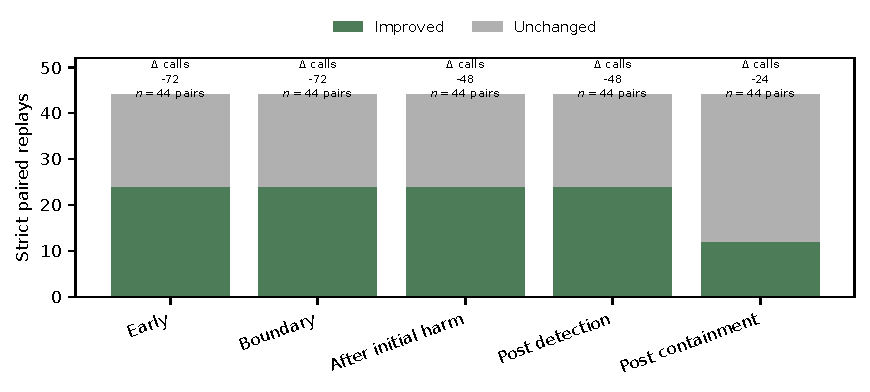
\includegraphics[width=\textwidth]{live-replay-treatments}
\caption{Strict replay results by action-relative delivery placement. Early and boundary treatments share the tested discrete preauthorization region.}
\label{fig:replay-timing}
\end{figure*}

\subsection{Post-denial substitution replay}

The separately rooted post-denial substitution study compares receiver-local strategies through the same TCOP acceptance boundary. It holds \AdaptiveStrictEpisodes{} policy-conditioned replay episodes fixed across \AdaptiveInitialBlocked{} frozen traces per policy. Every imported-evidence policy blocks the initial exact-bound action; \AdaptiveEligibleHarmfulBranches{} traces then have an eligible harmful capability, session, or delegation substitution. Exact Binding (C2) permits all \AdaptiveCTwoPostDenialCompleted{} substitutions, whereas Arrival Guard (C1), Campaign Correlation (C2E), and Standing Guard (C3) block them. Campaign Correlation uses a predeclared receiver-local relation, not a sender-provided enforcement field. Each imported-evidence strategy forwards all \AdaptiveBenignFallbacks{} of \AdaptiveBenignFallbacks{} exercised predeclared safe fallback actions. These safe fallbacks are a distinct in-campaign benign-continuation branch that the frozen policies explicitly forward after the initial denial. They are not the same-risk outside-campaign benign population on which the frontier measures Arrival Guard and Standing Guard collateral restriction.

The study also retains \AdaptiveLiveEpisodes{} bounded reference-runtime episodes. The runtime follows a predeclared harmful substitution branch after denial in \AdaptiveLiveAdapted{} episodes and a safe fallback in \AdaptiveLiveDidNotAdapt{} episodes. These runtime observations establish branch representability in the evaluated environment. The strict replay supplies the policy-conditioned conformance result; neither component estimates behavior prevalence in deployment.

\paragraph{Campaign Correlation strategy frontier:}
The separately sealed frontier evaluates \FrontierEpisodes{} deterministic policy episodes over \FrontierHarmfulAttempted{} harmful and \FrontierBenignAttempted{} benign logical actions. Its composition is fixed before policy execution (Table~\ref{tab:c2e-frontier-composition}): exact-bound and non-exact harmful actions share the \texttt{sensitive-write} risk family; the latter carry a receiver-established session-lineage relation. The same-risk benign actions outside a campaign retain that risk family but have a receiver-local campaign miss. Arrival Guard and Standing Guard block the same harmful population but constrain \FrontierCOneBenignConstrained{} and \FrontierCThreeBenignConstrained{} benign actions; Exact Binding blocks only \FrontierCTwoHarmfulBlocked{} harmful actions. Campaign Correlation blocks all \FrontierCampaignHarmfulBlocked{} campaign-linked non-exact harmful substitutions and forwards all \FrontierOutsideCampaignBenignForwarded{} benign same-risk actions outside the campaign. The receiver policy contract permits a declared delegation edge, but this frontier exercises session lineage only. Invalid, expired, and replayed context is rejected. Valid sender-suggested-only context is monitor-only, and the study records \FrontierUnrelatedRestrictions{} unrelated restrictions.

\begin{table}[t]\centering\scriptsize
\caption{Receiver-local strategy frontier. The same 10 harmful and 20 benign logical actions are evaluated per policy; this is a deterministic reference-policy result.}
\begin{tabular}{@{}p{0.48\columnwidth}cc@{}}\toprule
Strategy & \shortstack{Harmful\\blocked} & \shortstack{Benign\\constrained} \\ \midrule
Local Only (C0) & \FrontierCZeroHarmfulBlocked/\FrontierHarmfulAttempted & \FrontierCZeroBenignConstrained/\FrontierBenignAttempted \\
Arrival Guard (C1) & \FrontierCOneHarmfulBlocked/\FrontierHarmfulAttempted & \FrontierCOneBenignConstrained/\FrontierBenignAttempted \\
Exact Binding (C2) & \FrontierCTwoHarmfulBlocked/\FrontierHarmfulAttempted & \FrontierCTwoBenignConstrained/\FrontierBenignAttempted \\
Campaign Correlation (C2E) & \FrontierCTwoEHarmfulBlocked/\FrontierHarmfulAttempted & \FrontierCTwoEBenignConstrained/\FrontierBenignAttempted \\
Standing Guard (C3) & \FrontierCThreeHarmfulBlocked/\FrontierHarmfulAttempted & \FrontierCThreeBenignConstrained/\FrontierBenignAttempted \\ \bottomrule
\end{tabular}\label{tab:c2e-frontier}\end{table}


\begin{table}[t]\centering\scriptsize
\caption{Campaign Correlation frontier input composition (artifact identifier C2E). The fixed population contains five traces in each principal scenario; session lineage is the only strong relation exercised in this frontier.}
\begin{tabular}{@{}p{0.52\columnwidth}rr@{}}\toprule
Fixed trace class & Harmful & Benign \\ \midrule
Exact-bound action & \FrontierExactBindingHarmful & 0 \\
Non-exact action with receiver session lineage & \FrontierLineageHarmful & 0 \\
Predeclared safe fallback after relation & 0 & \FrontierSafeFallbackBenign \\
Same-risk action outside campaign & 0 & \FrontierOutsideCampaignBenign \\
Unrelated subject, session, or resource & 0 & \FrontierUnrelatedBenign \\
Invalid relation & 0 & \FrontierInvalidRelationControls \\
Expired relation & 0 & \FrontierExpiredRelationControls \\
Replayed relation & 0 & \FrontierReplayedRelationControls \\
Sender-suggested-only relation & 0 & \FrontierSenderSuggestedRelationControls \\ \bottomrule
\end{tabular}\label{tab:c2e-frontier-composition}\end{table}


\begin{figure}[t]
\centering
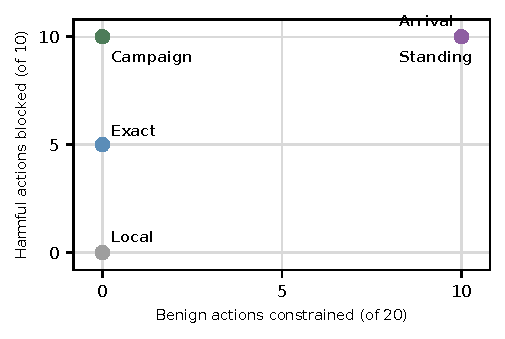
\includegraphics[width=0.94\columnwidth]{c2e-policy-frontier}
\caption{Receiver-local policy frontier in the sealed deterministic Campaign Correlation study. Arrival Guard and Standing Guard overlap at 10 benign actions constrained and 10 harmful actions blocked. The plotted points characterize configurable receiver strategies, not a mandatory TCOP response.}
\label{fig:c2e-policy-frontier}
\end{figure}

\subsection{Single-environment reference-path deployment}

The single-environment reference path runs \texttt{tcopd}-A, signed exchange, \texttt{tcopd}-B, the evaluator, and MCP gateway as separate processes on one host. It evaluates neither multi-host nor administrative separation. The \PhysicalFederationExchanges{} signed exchanges traverse both endpoints. Figure~\ref{fig:physical} separates prospective blocking from completed calls and later blocked opportunities. Each arm is one complete execution; harmful call attempts and signed exchanges are separate accounting units. Every gateway block cites Domain-B-local policy and decision provenance, establishing composition of this reference path.

\begin{figure}[t]
\centering
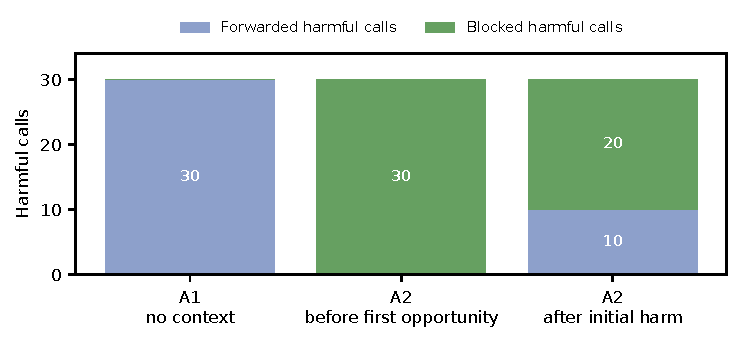
\includegraphics[width=\columnwidth]{physical-timing}
\caption{Single-environment reference-path timing result. The late arm separates already forwarded harmful calls from subsequent calls blocked by a Domain-B-local decision.}
\label{fig:physical}
\end{figure}

\begin{table}[t]\centering\small
\caption{Single-environment reference-path gateway arms. Each block is attributable to a Domain-B-local decision.}
\begin{tabular}{@{}p{0.40\columnwidth}rr@{}}\toprule
Arm & Forwarded & Blocked \\ \midrule
A1, no context & \AOneForwarded & 0 \\
A2, before first opportunity & 0 & \EarlyBlocked \\
A2, after initial harm & \LateForwarded & \LateBlocked \\ \bottomrule
\end{tabular}\label{tab:physical}\end{table}


\subsection{Measured scope}

The reported sub-millisecond values characterize the local deterministic harness. The single-environment reference-path deployment establishes that the tested relay, evaluator, and gateway adapter compose; strict replay supplies the controlled counterfactual. The timing treatments vary delivery relative to a receiver-local authorization boundary in synthetic action sequences. They do not reconstruct or draw measurements from a public incident.

\section{Security and Availability}

\subsection{Failure controls and receiver validation}

The evaluation injects invalid signature, wrong receipt, expiry, replay, unknown peer, disallowed import type, monitor-only policy, receiver unavailability, authorization timeout, restart, stale decision, session termination, and late-context conditions. In every tested condition, the receiver either rejects the context or applies its own disposition. Appendix~\ref{app:extended-results} reports the full source-control matrix; Table~\ref{tab:protocol-assurance} adds the validation-value mutation corpus.

The controls establish the boundary conditions for the result. A malformed or stale context does not create a restriction in the exercised path. A correlated but late context can be retained without being counted as prevention. A timeout or receiver outage resolves through Domain B's policy.

\subsection{Valid hostile peers}

Signature validation authenticates the issuer; it does not establish that the issuer's observation is true. The hostile-peer study therefore sends syntactically valid warnings from an authorized peer at increasing synthetic burst sizes. At the \HostileBurstWarnings-warning burst, the current containment-first policy accepts and constrains \HostileCurrentConstrained{} warnings. Idempotence accepts and constrains \HostileIdempotentConstrained{} warning while deduplicating \HostileIdempotentDeduplicated{}. The quota-plus-monitor response constrains \HostileQuotaConstrained{} warnings and monitors \HostileQuotaMonitored{}.

This result makes the receiver's policy choice explicit. A broad arrival-triggered guard can be used to impose availability cost, even when the peer is syntactically valid. Idempotence reduces repeated collateral restriction for a single warning. Quota-plus-monitor provides a measured overload posture in the tested burst: a receiver limits automatic restriction and retains excess warnings for local monitoring. The sweep is synthetic and does not estimate an operational warning rate.

\subsection{Security-availability trade-off}

Containment-first has a material availability cost in the selected synthetic false-warning treatments. In the inside-window early and boundary treatments, \InsideWindowBenignConstrained{} of \InsideWindowBenignAttempted{} benign agent calls are constrained and \InsideWindowWorkflowCompleted{} of \InsideWindowWorkflowTotal{} affected workflows complete. The remaining no-evidence and late treatments forward \OutsideWindowBenignForwarded{} of \OutsideWindowBenignAttempted{} benign agent calls and complete \OutsideWindowWorkflowCompleted{} of \OutsideWindowWorkflowTotal{} workflows. The aggregate \WorkflowCompleted{} of \WorkflowTotal{} result is reported for accounting, but does not blend away the treatment-specific false-warning cost.

\begin{figure}[t]
\centering
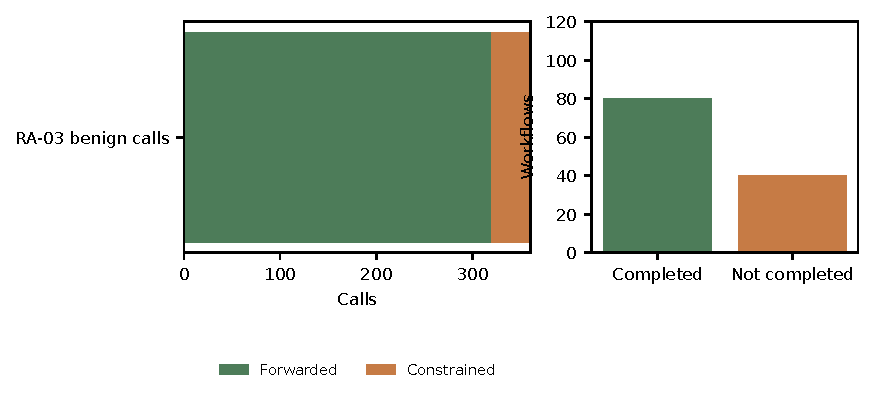
\includegraphics[width=\columnwidth]{security-availability}
\caption{Measured availability cost in the selected RA-03 synthetic workload.}
\label{fig:availability}
\end{figure}

\begin{table*}[t]\centering\scriptsize
\caption{Measured RA-03 availability cost under selected synthetic false-warning treatments and capability restriction; this is not a universal false-positive rate.}
\begin{tabular}{@{}p{0.22\textwidth}rrrp{0.23\textwidth}p{0.21\textwidth}@{}}\toprule
Treatment group & Attempted & Forwarded & Constrained & Workflow completion & Affected capability \\ \midrule
Inside-window early and boundary & \InsideWindowBenignAttempted & \InsideWindowBenignForwarded & \InsideWindowBenignConstrained & \InsideWindowWorkflowCompleted/\InsideWindowWorkflowTotal & repository.write in frozen benign metadata workflow \\
No context, outside window, post-detection, and post-containment & \OutsideWindowBenignAttempted & \OutsideWindowBenignForwarded & 0 & \OutsideWindowWorkflowCompleted/\OutsideWindowWorkflowTotal & no restriction in these treatments \\ \midrule
All selected treatments & \BenignAttempted & \BenignForwarded & \BenignConstrained & \WorkflowCompleted/\WorkflowTotal (\WorkflowCompletionRate) & selected synthetic capability restriction \\ \bottomrule
\end{tabular}\label{tab:utility}\end{table*}


The reported cohort establishes a bounded receiver-strategy frontier. Never restricting forwards the selected benign workload. Standing Guard maximizes blocking but constrains the capability continuously. Arrival Guard activates the same class-wide guard after accepted context becomes actionable. Exact Binding preserves containment on the accepted exact-binding subset while narrowing the restriction to that binding. The post-denial substitution and frontier studies add Campaign Correlation, which covers the declared related substitutions that Exact Binding alone permits.

\subsection{External-warning coverage and admission}

A credential-free successor evaluates the complete sealed external ledger from the pinned AgentDojo commit \cite{agentDojo} and pinned Prompt Guard 2 86M output configuration \cite{promptGuardTwo}; it consumes preserved detector outputs rather than rerunning the detector. Its declared normalizer maps \texttt{LABEL\_0} to no warning and \texttt{LABEL\_1} to a TCX prompt-attack category. Table~\ref{tab:independent-warning-full-pipeline} separates source coverage, detector output, normalization, receiver admission, and exact binding. Of \ExternalWarningFullAttackCases{} attack-bearing source cases, \ExternalWarningFullWarnings{} produce a warning and an admitted exact binding; \ExternalWarningFullAttackNoWarning{} produce no warning and therefore no actionable TCOP evidence. TCOP cannot compensate for a detector no-warning result.

Table~\ref{tab:independent-warning-full-outcomes} reports every policy over all \ExternalWarningFullSourceCases{} external source cases. Arrival Guard, Exact Binding, and Campaign Correlation block \ExternalWarningFullCTwoBlocked{} of \ExternalWarningFullAttackCases{} harmful actions, the \ExternalWarningFullConditionalNumerator{} for which accepted exact evidence exists, and forward the remaining \ExternalWarningFullCTwoForwarded{} no-warning harmful actions. They forward all \ExternalWarningFullBenignCases{} benign no-warning actions. Standing Guard blocks \ExternalWarningFullCThreeBlocked{} of \ExternalWarningFullAttackCases{} harmful actions but constrains all \ExternalWarningFullCThreeBenignConstrained{} of \ExternalWarningFullBenignCases{} benign actions because it is a standing receiver guard. This is an integration and authorization-coverage result, not an estimate of detector quality, warning prevalence, or deployment effectiveness.

Table~\ref{tab:independent-warning-v2-controls} adds deliberately derived protocol controls to the selected external bases. Exact Binding and Campaign Correlation apply no restriction to partial or mismatched bindings. Stale and replayed context are rejected before policy. Sender-suggested-only relation information remains nonrestrictive under Campaign Correlation. Campaign Correlation forwards all \ExternalWarningVTwoNoRelationCTwoEForwarded{} harmful substitutions without a receiver-created relation, including \ExternalWarningVTwoSessionNoRelationForwarded{} session-lineage and \ExternalWarningVTwoDelegationNoRelationForwarded{} delegation variants; it blocks all \ExternalWarningVTwoWithRelationCTwoEBlocked{} paired substitutions when the receiver has created the corresponding local relation. These controls demonstrate the declared receiver logic, not a general claim about correlation quality.

\begin{table}[t]\centering\scriptsize
\caption{Full external-warning pipeline coverage. All \ExternalWarningFullSourceCases{} cases in the sealed detector-output ledger are evaluated; a warning is not a detector-quality estimate.}
\begin{tabular}{@{}p{0.62\columnwidth}r@{}}\toprule
Stage or source category & Cases \\ \midrule
Attack-bearing source cases & \ExternalWarningFullAttackCases \\
\quad Detector warning $\rightarrow$ normalized TCX $\rightarrow$ admitted exact binding & \ExternalWarningFullWarnings/\ExternalWarningFullNormalized/\ExternalWarningFullAdmitted \\
\quad Detector no-warning $\rightarrow$ no actionable TCOP evidence & \ExternalWarningFullAttackNoWarning \\
Benign source cases, all detector no-warning & \ExternalWarningFullBenignCases \\
Total no actionable evidence & \ExternalWarningFullNoActionable \\ \bottomrule
\end{tabular}\label{tab:independent-warning-full-pipeline}\end{table}

\begin{table*}[t]\centering\scriptsize
\caption{Full-population receiver authorization outcomes over \ExternalWarningFullAttackCases{} attack-bearing and \ExternalWarningFullBenignCases{} benign external source cases. Arrival Guard, Exact Binding, and Campaign Correlation use accepted evidence conditionally; Standing Guard is a standing local restriction.}
\begin{tabular}{@{}lrr|rr@{}}\toprule
Policy & \shortstack{Harmful\\blocked} & \shortstack{Harmful\\forwarded} & \shortstack{Benign\\constrained} & \shortstack{Benign\\forwarded} \\ \midrule
Local Only (C0) & \ExternalWarningFullCZeroBlocked/\ExternalWarningFullAttackCases & \ExternalWarningFullCZeroForwarded/\ExternalWarningFullAttackCases & \ExternalWarningFullCZeroBenignConstrained/\ExternalWarningFullBenignCases & \ExternalWarningFullCZeroBenignForwarded/\ExternalWarningFullBenignCases \\
Arrival Guard (C1) & \ExternalWarningFullCOneBlocked/\ExternalWarningFullAttackCases & \ExternalWarningFullCOneForwarded/\ExternalWarningFullAttackCases & \ExternalWarningFullCOneBenignConstrained/\ExternalWarningFullBenignCases & \ExternalWarningFullCOneBenignForwarded/\ExternalWarningFullBenignCases \\
Exact Binding (C2) & \ExternalWarningFullCTwoBlocked/\ExternalWarningFullAttackCases & \ExternalWarningFullCTwoForwarded/\ExternalWarningFullAttackCases & \ExternalWarningFullCTwoBenignConstrained/\ExternalWarningFullBenignCases & \ExternalWarningFullCTwoBenignForwarded/\ExternalWarningFullBenignCases \\
Campaign Correlation (C2E) & \ExternalWarningFullCTwoEBlocked/\ExternalWarningFullAttackCases & \ExternalWarningFullCTwoEForwarded/\ExternalWarningFullAttackCases & \ExternalWarningFullCTwoEBenignConstrained/\ExternalWarningFullBenignCases & \ExternalWarningFullCTwoEBenignForwarded/\ExternalWarningFullBenignCases \\
Standing Guard (C3) & \ExternalWarningFullCThreeBlocked/\ExternalWarningFullAttackCases & \ExternalWarningFullCThreeForwarded/\ExternalWarningFullAttackCases & \ExternalWarningFullCThreeBenignConstrained/\ExternalWarningFullBenignCases & \ExternalWarningFullCThreeBenignForwarded/\ExternalWarningFullBenignCases \\ \bottomrule
\end{tabular}\label{tab:independent-warning-full-outcomes}\end{table*}

\begin{table}[t]\centering\scriptsize
\caption{Independent Warning Admission v2 derived controls. Each row contains \ExternalWarningVTwoSelectedPositive{} derived cases. The substitution rows contain \ExternalWarningVTwoSessionNoRelationForwarded{} session-lineage and \ExternalWarningVTwoDelegationNoRelationForwarded{} delegation variants.}
\begin{tabular}{@{}p{0.51\columnwidth}p{0.38\columnwidth}@{}}\toprule
Control & Receiver result \\ \midrule
Partial binding & Exact Binding/Campaign Correlation: \ExternalWarningVTwoPartialCTwoERestricted/\ExternalWarningVTwoSelectedPositive{} restrictions \\
Mismatched binding & Exact Binding/Campaign Correlation: \ExternalWarningVTwoMismatchCTwoERestricted/\ExternalWarningVTwoSelectedPositive{} restrictions \\
Stale or replayed context & Campaign Correlation: \ExternalWarningVTwoStaleCTwoERejected/\ExternalWarningVTwoSelectedPositive{} rejected before policy \\
Sender-suggested-only relation & Campaign Correlation: \ExternalWarningVTwoSenderSuggestedCTwoERestricted/\ExternalWarningVTwoSelectedPositive{} restrictions \\
Harmful substitution, no B-local relation & Campaign Correlation: \ExternalWarningVTwoNoRelationCTwoEForwarded/\ExternalWarningVTwoSelectedPositive{} forwarded \\
Harmful substitution, B-local relation & Campaign Correlation: \ExternalWarningVTwoWithRelationCTwoEBlocked/\ExternalWarningVTwoSelectedPositive{} blocked \\ \bottomrule
\end{tabular}\label{tab:independent-warning-v2-controls}\end{table}


\subsection{Local overhead}

The performance experiment reports authorization, gateway, and warning-to-enforcement measurements separately for cache-disabled and fixed-time-to-live cache selections. The correctness and causal replays use the cache-disabled configuration. The local-harness measurements appear in Appendix~\ref{app:extended-results}.

\section{Related Work}

\subsection{Threat-intelligence exchange}

STIX/TAXII, MISP, and DShield distribute threat information \cite{stix21,taxii21,mispCore,dshieldFeeds}. TCOP may ingest evidence derived from them; it addresses the later agent-runtime question of whether a receiver should authorize one pending tool or capability action after receipt-, session-, and action-specific validation. These systems do not specify that action-time receiver-local authorization contract.

\subsection{Response orchestration}

RID, DOTS, and OpenC2 exchange incident reports, mitigation signals, and defense commands \cite{rid12,dots21,openc2v1}. CACAO and SOAR coordinate playbooks and response workflows \cite{cacao20,bridges23}. Either can implement a response after TCX acceptance. TCOP instead bounds the preceding decision input: whether signed runtime evidence applies to one pending receiver-side agent action. Course of action, workflow execution, and enforcement remain receiver-local.

\subsection{Trust, identity, and local policy}

KeyNote and macaroons support delegated authorization \cite{keynote99,birgisson2014macaroons}; TCX instead carries behavioral runtime evidence into a locally created decision. This avoids imported evidence becoming ambient enforcement authority, related to the confused-deputy concern \cite{hardy88}. Zero trust separates policy decision from enforcement \cite{nistZta}; SPIFFE federation authenticates foreign workloads \cite{spiffeFederation}; and RATS separates evidence, appraisal, verifier, and relying party \cite{rats}. TCOP applies those separations to cross-domain agent actions: it combines authenticated peer identity with receiver-local correlation and appraisal. Collaborative intrusion detection identifies relevant coordination and adversarial-participant questions \cite{bye2010}; the central audit here is only a bounded fact-equivalent control.

\subsection{Agent interoperability and tool protocols}

MCP standardizes client access to server tools and resources \cite{mcpAuthorization}; its gateway is the reference tool-call enforcement point here. A2A standardizes independent-agent discovery and collaboration \cite{a2aSpec}, and ANP addresses agent-network communication and discovery \cite{anpSpec}. They can supply transport or session context. Table~\ref{tab:protocol-comparison} summarizes the contract-level distinction: TCOP adds receipt-bound validation of signed runtime evidence against a pending receiver-side agent action, while leaving response selection and enforcement with the receiver.

\subsection{Agent and tool security}

Prompt injection and tool-integrated agents motivate the synthetic scenarios. Liu et al. benchmark prompt-injection attacks and defenses, while InjecAgent evaluates indirect injection against tool-integrated agents \cite{liu2024prompt,zhan2024injecagent}. TCOP does not compete with those detectors. It evaluates whether externally observed runtime evidence can affect a locally governed pending action in time.

\section{Limitations and Conclusion}

\subsection{Limitations}

The claim boundary in Section~2 and Table~\ref{tab:limitations} applies throughout. The evidence uses synthetic agent tools and scenarios, receipt-based correlation, one reference gateway, local-harness performance, and one frozen model/runtime selection. The post-denial substitution study evaluates predeclared branches in a bounded reference runtime, not deployment prevalence. The Campaign Correlation frontier establishes selectivity only for its declared deterministic receiver-local strategy, not a general escalation policy or deployment effectiveness. The full external-warning study consumes preserved detector outputs for \ExternalWarningFullSourceCases{} source cases: \ExternalWarningFullWarnings{} produce admitted exact evidence and \ExternalWarningFullAttackNoWarning{} attack-bearing cases produce no warning. It does not estimate detector quality, warning prevalence, arbitrary warning-source behavior, or production effectiveness. The protocol lifecycle lacks evidence for key rotation, revocation propagation, heterogeneous federation deployment, and cross-host transport delay.

The validation-value study establishes a precise, narrow result. Its protected population contains \MatchingHarmfulActions{} accepted binding-matched harmful actions. C1-class and C2 both block those actions, while C2 avoids the \COneClassBenignConstrained{} benign constraints observed under C1-class. Across the full cohort, C1-class blocks \COneClassHarmfulBlocked{} of \ValidationEpisodes{} harmful actions and C2 blocks \CTwoHarmfulBlocked{}; C2 rejects mismatched, expired, replayed, or uncorrelated warnings rather than applying a broad class guard. The hostile-peer, correlation, and mutation studies are deterministic synthetic sweeps. They establish behavior in the examined reference path rather than a field prevalence estimate.

The retained amendment history makes the RA-03 eligibility correction visible. Table~\ref{tab:ra03-eligibility} reports the before-and-after rule outcomes. The correction affects the benign availability cohort; the strict deterministic causal comparison excludes RA-03 and remains separately rooted.

\subsection{Conclusion}

TCOP specifies an evidence-to-authorization boundary at which cross-domain runtime evidence becomes an input to a receiver's local authorization decision for a pending agent action. The main result is conditional on timeliness: when accepted evidence reaches the receiver inside an action's containment window, it can alter locally governed enforcement and reduce later harmful agent-action opportunities. TCOP specifies authenticated evidence exchange, receiver acceptance, and the authority boundary. It does not prescribe Exact Binding, Campaign Correlation, monitoring, or a standing guard. In every tested single-environment reference-path and replay condition, gateway blocks cite receiver-local policy and decision records.

The validation-value study shows why the full evidence binding matters. On the accepted binding-matched harmful population, validated matching preserves the class guard's containment while avoiding its measured collateral benign constraints. The post-denial substitution and Campaign Correlation frontier studies show alternative receiver strategies supported by the same boundary: Exact Binding prioritizes precision, while the evaluated Campaign Correlation strategy covers the declared related substitutions and forwards the measured outside-campaign same-risk actions. The external-warning study separates source coverage from authorization: after declared normalization and local receipt construction, receiver policies act on accepted evidence, while no-warning cases remain outside conditional TCOP coverage. The artifact preserves the source roots, exclusions, sealed study plans, normalized data, and regenerated figures and tables so reviewers can inspect each current claim against its evidence.

\bibliographystyle{plain}
\bibliography{references}
\appendix
\section{Open Science Appendix}

\ifdefined\TCOPPreprint The source and artifacts are available at\else The anonymous artifact accompanies the submission at\fi\ \TCOPArtifactLink{}. It contains the paper source, source-verification reports, normalized data, figure and table sources, expected results, claim and number audits, a compact reviewer package, the sealed TCX Validation-Value Study v2, Post-Denial Substitution Study v1, Campaign Correlation Frontier Study v1 (artifact identifier C2E), Independent Warning Admission v2 external-stratified study, and the full-population external-warning successor. The predecessor roots remain unchanged for lineage. It contains no provider credentials, production credentials, personal paths, or unpublished incident data.

The artifact is organized around four reproduction tiers. Tier 0 verifies immutable roots, normalizes data, regenerates figures and tables, audits manuscript numbers and anonymity, and builds the paper. Tier 1 reruns the deterministic causal core without external credentials. Tier 2 strictly replays frozen agent traces through local-only and TCOP treatments without model credentials. Tier 3 is an optional credentialed regeneration of live traces and is not required for the causal findings.

The default reviewer command runs Tier 0 plus strict agent replay without reading a model-provider environment variable. The validation-value study is credential-free and includes its sealed output, pre-analysis plan, expected results, mutation corpus, and two byte-identical clean rerun report. The post-denial substitution, Campaign Correlation, and independent-warning studies include sealed plans, normalized summaries, source manifests, candidate and selection ledgers where applicable, and dedicated verifier commands documented in the anonymous artifact. The expected-results manifest records the strict-pair counts, single-environment reference-path arms, control outcomes, strategy digests, source roots, validation-value results, and all study results used by the manuscript.

The artifact uses Python, the TCOP CLI, Matplotlib for vector figures, and a TeX distribution for the PDF. Docker is required only for the optional reference-gateway smoke path, which also requires a separately supplied pinned gateway checkout. The source-verification report records the formal amendment that admits the available deterministic evidence root in place of an unavailable predecessor root.

Tier 0, Tier 1, Tier 2, and the validation-value verifier complete without provider credentials. Tier 3 documents its provider/runtime lock, eligibility criteria, bounded attempts, expected variability, and cost category separately from frozen-trace reproduction. A fresh provider run is not permitted to replace the replay evidence used for the paper's causal claims.

\section{Ethics Appendix}

All evaluated tools and target systems are synthetic. No production credentials, real repositories, customer systems, datasets, or workloads were attacked. Prompts and tool calls are restricted to a test environment, and no autonomous production enforcement occurred. The credentialed model activity was bounded by synthetic tool interfaces. No human subjects were involved, and the study does not collect or release personal data.

The work concerns defensive handling of potentially harmful tool calls. An executable gateway and replay environment could be misused if presented as a way to control another domain. The artifact reduces this risk through synthetic inputs, omitted target infrastructure and credentials, and a receiver-local authorization boundary. The evaluated protocol does not export a remote enforcement interface or a production attack path.

False or malicious warnings are the principal ethical and operational risk. The paper therefore reports both the benign-workflow disruption caused by containment-first restriction and the valid-hostile-peer burst results. A receiver decides whether to restrict, monitor, deduplicate, or rate-limit a warning. This cost and responsibility remain part of the design result.

The public incident is a motivation for the cross-domain failure pattern, not an attribution or empirical reconstruction.

\section{Frozen Strategy Details}

The study certifies four objective-specific frozen configurations: containment-first, balanced federated, utility-preserving, and forensic-oriented. The paper's primary causal deterministic comparison uses containment-first because it is the configuration with matched local-policy pairs. Balanced and utility configurations are retained in the artifact but their unmatched comparisons are excluded from the causal claim. Artifact configuration identifiers remain in the machine-readable strategy manifest.

The full manifest digests and certification status appear in the source-verification report and normalized strategy records. The paper does not portray the forensic configuration as a separable composable overlay, and it makes no unsupported reconstruction-quality claim.

\section{Live Amendment History}

The live evaluation preserves a visible sequence of sealed artifacts. The earliest provider-failure artifacts remain negative results. Amendments correct provider transport compatibility, align frozen benign eligibility, correct an artifact completion gate, reconcile a derived utility counter from immutable replay rows, and add the reference-path origin relay without new model sampling. The immutable historical artifact identifier retains its original end-to-end label. None changes TCX fields, receiver-local policies, scenario prompts, tools, treatment definitions, or frozen traces.

\begin{table*}[t]\centering\scriptsize
\caption{Live runtime amendment history. Digest prefixes identify the immutable predecessor and successor roots; full digests are retained in the normalized amendment-chain data and source-verification report. The first two predecessor artifacts are retained provider-failure negatives.}
\begin{tabular}{@{}p{0.07\textwidth}@{\hspace{0.2em}}p{0.16\textwidth}@{\hspace{0.2em}}p{0.09\textwidth}@{\hspace{0.2em}}p{0.07\textwidth}@{\hspace{0.2em}}p{0.08\textwidth}@{\hspace{0.2em}}p{0.09\textwidth}@{\hspace{0.2em}}p{0.12\textwidth}@{\hspace{0.2em}}p{0.12\textwidth}@{}}\toprule
Amendment & Cause & Model sampling? & Traces? & Protocol / policy? & Result derivation? & Predecessor digest & Successor digest \\ \midrule
001 & Provider completion-token field & No successful sampling & No & No & No & e5cf49806b70 & 698ca3c116af \\
002 & Provider reasoning mode & No & No & No & No & 698ca3c116af & f9bccfcaeff8 \\
003 & RA-03 eligibility aligned to frozen truth & Yes, eligible cohort capture & No & No & Eligibility only & f9bccfcaeff8 & cebc669a7a3c \\
004 & Completion-gate ordering & No & No & No & No & cebc669a7a3c & 24a20e9c48a2 \\
005 & Derived utility reconciliation & No & No & No & Yes, replay-row aggregation & 24a20e9c48a2 & 2b1f92ff4481 \\
006 & End-to-end tcopd-a relay replay & No & No & No & Reference-deployment evidence & 2b1f92ff4481 & 546f3547b727 \\ \bottomrule
\end{tabular}\label{tab:amendments}\end{table*}


\subsection{RA-03 eligibility correction}

Amendment 003 corrected an eligibility implementation that applied a global high-risk capability rule to the benign RA-03 metadata-write workflow. The frozen benchmark had already declared \texttt{repository.write} permitted for that workflow. The original and corrected rules, as well as their distinct retained trace-eligibility reports, are included in the artifact. Table~\ref{tab:ra03-eligibility} gives the sensitivity view required to distinguish a trace-eligibility correction from a changed harmful-action result.

\begin{table}[t]\centering\scriptsize
\caption{RA-03 eligibility correction. The amended rule accepts the already frozen benign metadata capability; deterministic causal counts do not use RA-03.}
\begin{tabular}{@{}p{0.47\columnwidth}rr@{}}\toprule
Rule & Attempts & Eligible \\ \midrule
Pre-correction global rule & \RAThreeBeforeAttempts & \RAThreeBeforeEligible \\
Amendment 003 permitted-capability rule & \RAThreeAfterAttempts & \RAThreeAfterEligible \\ \bottomrule
\end{tabular}\label{tab:ra03-eligibility}\end{table}


\begin{figure*}[t]
\centering
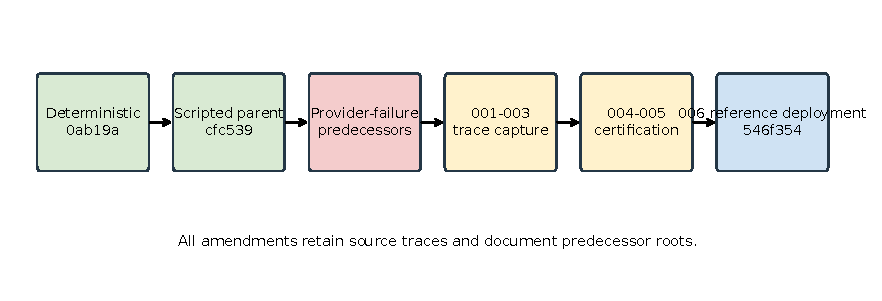
\includegraphics[width=\textwidth]{artifact-lineage}
\caption{Artifact and amendment lineage. Short prefixes identify roots; the source-verification report records full digests and predecessor links.}
\label{fig:lineage}
\end{figure*}

\section{Extended Results}
\label{app:extended-results}

\begin{table*}[t]\centering\small
\caption{What the evaluation supports and does not support.}
\begin{tabular}{p{0.3\textwidth}p{0.6\textwidth}}\toprule
Evidence & Supported scope \\ \midrule
Deterministic matched pairs & Causal comparison under matched frozen local policy and synthetic scenarios \\
Executable replay & Exact captured action-sequence comparison without model credentials \\
Live trace generation & A bounded credentialed cohort generated action attempts \\
Single-environment reference-path deployment & A signed tcopd-A-to-tcopd-B path and receiver-local gateway decisions in one reference environment \\
Validation-value and assurance cohort & Semantic binding and executed receiver-validator mutations; hostile-peer and correlation tables are formula-computed illustrations \\
Post-denial substitution replay & Policy-conditioned post-denial branches in a bounded reference runtime, not deployment prevalence \\
Campaign Correlation frontier & Deterministic receiver-local Campaign Correlation selectivity, not a general escalation policy or deployment-effectiveness estimate \\
Full external-warning ledger & All 168 sealed external source cases: 25 accepted exact bindings, 47 attack-bearing no-warning cases, and 96 benign no-warning cases; authorization coverage, not detector-quality evidence \\
Not established & Production deployment, Internet-scale federation, key-lifecycle operation, uninstrumented incidents, or universal superiority to central defense \\ \bottomrule
\end{tabular}\label{tab:limitations}\end{table*}


The normalized data preserves the full strict-pair and treatment-level rows with source artifact digests, paths, and row identifiers. The timing result distinguishes delivery before the first harmful opportunity, at the first-action authorization boundary, after initial harm but before later actions, after receiver-local detection, and after partial local containment. No figure interpolates a causal effect between these measured placements.

\begin{table*}[t]\centering\small
\caption{Strict replay timing treatments. A treatment can be too late for one action while still affecting later opportunities.}
\begin{tabular}{@{}p{0.34\columnwidth}rrr@{}}\toprule
Action-relative placement & Improved & Unchanged & Harmful-action delta \\ \midrule
Before first harmful opportunity & 24 & 20 & -72 \\
At first-action authorization boundary & 24 & 20 & -72 \\
After initial harm, before later actions & 24 & 20 & -48 \\
After receiver-local detection & 24 & 20 & -48 \\
After partial local containment & 12 & 32 & -24 \\ \bottomrule
\end{tabular}\label{tab:timing}\end{table*}


\begin{table*}[t]\centering\scriptsize
\caption{Negative and failure controls. Ten controls (NC-01--04, NC-07, NC-10--12, NC-14, NC-16) were executed and passed in the sealed live artifact. NC-05 and NC-09 are covered by executed signed-envelope mutations in \protect\path{artifacts/tcx-validation-value-v2/property-test-report.json} (\texttt{issuer} and \texttt{action\_semantic}, respectively), not by live injections. Four rows (NC-06, NC-08, NC-13, NC-15) were recorded as passed in the sealed live artifact without executing the condition; they are untested design properties, not results. See the artifact's known-issues file, \protect\path{docs/KNOWN_ISSUES.md}.}
\begin{tabular}{@{}p{0.15\textwidth}@{\hspace{0.7em}}p{0.20\textwidth}@{\hspace{0.7em}}p{0.20\textwidth}@{\hspace{0.7em}}p{0.12\textwidth}@{\hspace{0.7em}}p{0.08\textwidth}@{\hspace{0.7em}}p{0.18\textwidth}@{}}\toprule
Condition & Expected behavior & Observed behavior & Invariant & Pass & Source / evidence \\ \midrule
Invalid signature & Reject before restriction & Rejected; no restriction & Signed input & Yes & NC-01; live executed \\
Wrong receipt & Reject before restriction & Rejected; no restriction & Receipt correlation & Yes & NC-02; live executed \\
Expired context & Reject before restriction & Rejected; no restriction & Bounded freshness & Yes & NC-03; live executed \\
Replayed context & Reject before restriction & Rejected; no restriction & Replay protection & Yes & NC-04; live executed \\
Unknown peer & Reject before restriction & identity\_{}unknown; no restriction & Authorized peer & Yes & NC-05; mutation: issuer \\
Disallowed import type & Reject before restriction & Not executed; design property & Context class & Not tested & NC-06; not executed \\
Monitor-only policy & Do not preempt first call & First call not blocked & Local detection timing & Yes & NC-07; live executed \\
No remote enforcement & Never accept remote enforcement & Not executed; design property & Receiver authority & Not tested & NC-08; not executed \\
Remote TCX action & Never interpret remote action & Remote fields action and enforcement ignored & Receiver authority & Yes & NC-09; mutation: action\_{}semantic \\
Gateway cache disabled & Evaluate each authorization & Cache disabled & Replay correctness & Yes & NC-10; live executed \\
tcopd B unavailable & Use B-local disposition & Local fail-closed policy & Receiver authority & Yes & NC-11; live executed \\
Authorization timeout & Use B-local disposition & Sender does not choose timeout & Receiver authority & Yes & NC-12; live executed \\
Gateway restart & Recompute local state & Not executed; design property & Receiver authority & Not tested & NC-13; not executed \\
Stale decision & Recompute local state & Fresh decision used & Receiver authority & Yes & NC-14; live executed \\
Session termination before arrival & Do not cross sessions & Not executed; design property & Session binding & Not tested & NC-15; not executed \\
Arrival after local containment & No reversal of completed action & Non-preventive late context & Containment window & Yes & NC-16; live executed \\ \bottomrule
\end{tabular}\label{tab:controls}\end{table*}


\begin{table*}[t]\centering\small
\caption{Local harness performance. These deterministic local measurements characterize implementation overhead in the test harness and are not production inter-domain latency estimates.}
\begin{tabular}{lrrrr}\toprule
Selection & Authorization p95 (ms) & Gateway p95 (ms) & Warning-to-enforcement p95 (ms) & Cache hit rate \\ \midrule
Disabled & 0.020 & 0.025 & 0.33 & 0.00 \\
Enabled, fixed 5s TTL & 0.00067 & 0.027 & 0.33 & 0.95 \\ \bottomrule
\end{tabular}\label{tab:performance}\end{table*}


The selected utility result is intentionally reported alongside security benefit. Restriction expiry and recovery remain receiver-local, and the artifact retains the raw treatment rows required to inspect the completion calculation.

\section{Failure-Control Detail}

The base control suite exercises invalid signatures, receipt mismatch, expiry, replay, unauthorized peers, unsupported imports, local monitor-only behavior, receiver unavailability, timeout, gateway restart, stale decisions, session binding, and late delivery. In every evaluated gateway block, the recorded provenance is Domain-B-local. The validation-value study adds mutation cases for signed-envelope fields and action-like metadata. The generated body tables provide the reader-facing summary; normalized rows preserve each source record.

\section{Reproducibility Details}

The default reviewer workflow avoids live credentials. It verifies source roots, regenerates all paper-local derivatives, and invokes strict replay on frozen traces. Exact expected counts and full source digests are machine-checkable in the \TCOPArtifactDescription{} manifest. The deterministic causal-core tier writes a new output root and compares its declared deterministic results; it never overwrites the sealed sources.

The live provider environment is documented only for optional trace regeneration. A current provider response can differ from the frozen cohort; such a replication does not replace the trace-replay evidence or modify the paper's claims.

\end{document}
